\section{Evaluation}
\label{s:eval}

This section empirically answers several questions:

\begin{CompactItemize}

\item Is \txn sophisticated enough to support real storage systems
  and to achieve good performance?  (\autoref{sec:eval:func})

% - Much higher absolute performance than DFSCQ.  Something like 3x on
%   smallfile.  Without bypass writes.  (Verifying Go code is better than
%   extracting Haskell.)

\item Is \txn's concurrency important for storage systems to achieve
  high performance?  (\autoref{sec:eval:concur})

% - Maybe some concurrency benefits?  Try putting a big lock around
%   everything in the big NFS server, and running on a real disk.

\item Are Perennial's verification techniques important for proving the
  correctness of \txn (\autoref{sec:eval:modular}) and for enabling
  application developers to prove their code on top of \txn
  (\autoref{sec:eval:atomic})?

% Case study of where we use crash locks, lifting,
% logically atomic crash specs

\item How much effort is required to prove the correctness of
  \txn and applications on top of \txn?  (\autoref{sec:eval:proof})

% Lines of proof for src/program_proofs (30x Go code size, approx)
% Split up GoTxn vs. simple-nfsd.

\item Does verification help developers avoid bugs?
  (\autoref{sec:eval:bugs})

% Case study 1:
% - mundane bugs in simple-nfsd
% - absorption bug in wal??

% Case study 2:
% - concurrency (or other) bugs in jbd2

\end{CompactItemize}


\subsection{\txn is functional and performant}
\label{sec:eval:func}

To evaluate whether \txn is sophisticated enough to support real storage systems
and to achieve good performance, we measure the performance of \gnfs using three
benchmarks: the LFS smallfile and largefile benchmarks, as well as a development
workload, consisting of running \cc{git clone} on the xv6 source-code
repository~\cite{xv6} and compiling it with \cc{make}. These benchmarks were
also used by DFSCQ~\cite{chen:dfscq}, a previous state-of-the-art verified
file system. As a comparison point for \gnfs, we run the Linux kernel NFS server
exporting an ext4 file system. The ext4 file system writes data through the
journal (using the \cc{data=journal} mount option), so that both systems provide
the same crash-safety guarantees. The GoJournal implementation supports atomic
but unstable writes, which match the semantics of unstable NFS \cc{WRITE}
operations. While all the internal layers of the proof support unstable writes,
the separation logic specification presented in \autoref{s:design} does not, so we conducted the
evaluation without using unstable writes in \gnfs.
% We evaluate the performance
% impact of these decisions on both ext4 and \gnfs.

We ran the benchmarks on Linux 5.12.3, using its NFS client to mount both \gnfs
and the Linux NFS server. The experiments are run on two machines, a desktop
with a relatively slow SSD and an EC2 machine with a fast NVMe disk. The
desktop has an Intel Xeon E5-2640 20-core CPU at 2.4~GHz, 64~GB of RAM,
and a 256~GB Samsung 850 PRO SSD, which we use to measure in-memory performance
with no disk bottleneck as well as the impact of relatively slow storage. The
EC2 instance is an i3.metal, which has 72 vCPUs, 512~GB of RAM, and a
local 1.9~TB NVMe SSD, which we use to measure performance on fast storage with
good random-access performance. To reduce variability we
limit the experiment to a single socket, disable turbo boost, disable processor
sleep states, and disable Spectre mitigations in the kernel.

\begin{figure}[ht!]
  \centering

  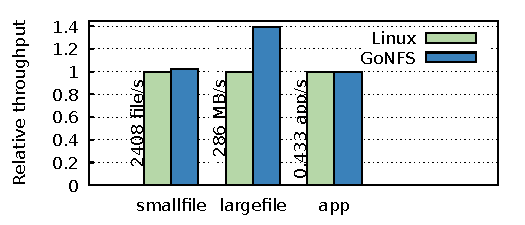
\includegraphics[scale=0.9]{fig/bench.pdf}

  \caption{Performance of Linux NFS and \txn + \gnfs for \cc{smallfile},
    \cc{largefile}, and \cc{app} workload, on a RAMdisk. On an NVMe disk \gnfs
    achieves at least 90\% of Linux's throughput.}
\label{fig:perf}
\end{figure}

% \begin{figure}[ht!]
%   \centering
%
%   \includegraphics[scale=0.9]{fig/bench-ssd.pdf}
%
%   \caption{Performance of Linux NFS and \txn + \gnfs for \cc{smallfile},
%     \cc{largefile}, and \cc{app} workload, on a (slow) SSD.}
% \label{fig:perf-ssd}
% \end{figure}

\begin{figure}[ht!]
  \centering

  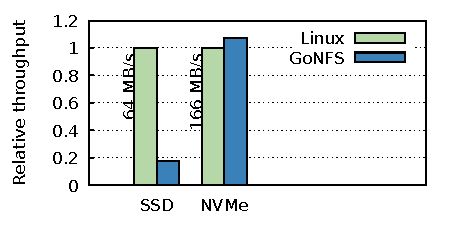
\includegraphics[scale=0.9]{fig/largefile-alt.pdf}
  \caption{Performance of \cc{largefile} depends on the storage medium. Linux
    takes advantage of unstable writes to write a large amount of data between
    barriers but \gnfs flushes to disk frequently.}
  %\caption{Performance of \cc{largefile} on a slow SSD across a few
  %  configurations. \tej{I wanted a cluster per configuration, and colors to
  %    correspond to the system.}}
\label{fig:largefile}
\end{figure}

% \begin{figure}[ht!]
%   \centering
%
%   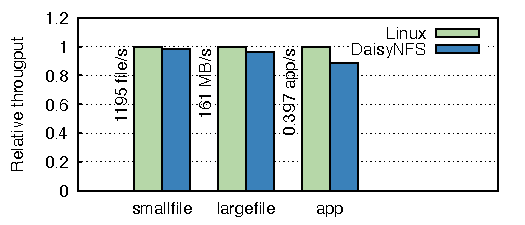
\includegraphics[scale=0.9]{fig/aws/bench.pdf}
%
%   \caption{Performance of Linux NFS and \txn + \gnfs for \cc{smallfile},
%     \cc{largefile}, and \cc{app} workload, on a RAMdisk. \joe{This was run on an
%       AWS i3.metal with a Go in-memory disk.}}
% \label{fig:perf-aws}
% \end{figure}
%
% \begin{figure}[ht!]
%   \centering
%
%   \includegraphics[scale=0.9]{fig/aws/bench-ssd.pdf}
%
%   \caption{Performance of Linux NFS and \txn + \gnfs for \cc{smallfile},
%     \cc{largefile}, and \cc{app} workload, on a fast NVMe SSD. \joe{This was run
%       on an AWS i3.metal.}}
% \label{fig:perf-aws-ssd}
% \end{figure}

We first evaluate \gnfs's performance with a single client issuing requests.
\autoref{fig:perf} shows the results on the Intel Xeon desktop with both file systems backed by RAM, to
avoid any I/O overhead --- \gnfs takes a simple Go interface for the disk, which
we implemented with a large array, while ext4 uses a file in
tmpfs.\footnote{Running \gnfs on tmpfs performs slightly worse due to the around
  1 microsecond syscall overhead of each disk operation, which ext4
  does not incur since everything happens within the kernel.} \gnfs achieves at
least the throughput of ext4 across the different workloads.

On both the NVMe and slower SSD, \txn's performance relative to ext4 is similar on the \cc{smallfile} and \cc{app} workloads (not plotted),
again achieving at least 90\% of the throughout of ext4.
%
% next consider the effects of I/O overhead on disks. For the
% \cc{smallfile} and \cc{app} workloads, \txn's performance relative to ext4
% on both the NVMe and slower SSD is similar to ramdisk,
However, \gnfs performance on the \cc{largefile} benchmark is sensitive to disk I/O characteristics,
as shown in \autoref{fig:largefile}. On the faster NVMe device, \gnfs's large file performance
is comparable to ext4's, but on the slower SSD, it drops to under 20\% of ext4's throughput.
The reason is that the \cc{largefile}
benchmark produces a large number of parallel, unstable writes to the same file.
\gnfs runs them sequentially due to a per-inode lock, and then journals sequentially because it
ignores the unstable write flag. A disk barrier on the SSD takes about 2
milliseconds, so getting good disk throughput requires writing a large amount of
data before issuing a barrier, and the 64~KB batch size is insufficient to get
the maximum SSD write throughput. Re-running the experiment with
unstable writes enabled in \gnfs raises its throughput to 90\% of ext4's.

% The figure shows that \gnfs achieves
% comparable performance when using unstable writes, because even though the
% writes are issued sequentially \txn commits them to disk in large batches. Both
% systems get the same low performance if the benchmark is changed to consist of
% sequential, stable writes with the NFS client's \cc{sync} mount option, causing
% ext4's journaling behavior to match \gnfs in order to guarantee each write is
% persisted before the next is issued.

% shows the relative performance on this workload.

% \ralf{Are we switching to a different figure here?
% Namely Figure 19, which the comment says we will cut?}
% When run on a fast NVMe disk, relative
% performance is nearly identical. \tej{James suggested using the NVMe numbers as
% the main results and mentioning RAMdisk in passing.} \gnfs is able to achieve 90--95\% of the
% throughput of ext4 across the different workloads. We expect \gnfs and \txn to
% be somewhat slower, because they are written in Go rather than C, but \txn does
% implement sophisticated performance optimizations such as in-place updates of
% buffers, full-block overwrites without read-modify-write, etc. This suggests
% that \txn is a realistic journaling system for performant storage applications.
%
% On an SSD, \txn gets comparable performance for the \cc{smallfile} and \cc{app}
% benchmarks but is slower than Linux for the \cc{largefile} benchmark, as seen in
% \autoref{fig:perf-ssd} which shows relative throughput on the same benchmarks as
% \autoref{fig:perf} but on an SSD instead of a RAMdisk. We further explored the
% performance of this benchmark by running a number of other configurations, shown
% in \autoref{fig:largefile}. The \cc{largefile}
% benchmark produces a large number of parallel writes to the same file, which
% \gnfs runs sequentially due to a per-inode lock and journals sequentially due to
% the use of stable writes. The SSD can get 150 MB/s with sequential writes, but
% this requires writing a large amount of data before issuing a disk barrier,
% larger than the 64~KB write batch size. The figure shows that \gnfs achieves
% comparable performance when using unstable writes, because even though the
% writes are issued sequentially \txn commits them to disk in large batches. Both
% systems get the same low performance if the benchmark is changed to consist of
% sequential, stable writes with the NFS client's \cc{sync} mount option, causing
% ext4's journaling behavior to match \gnfs in order to guarantee each write is
% persisted before the next is issued.
% increasing the write batch size further to 128~KB also improves performance.

%\mfk{this paragraph doesn't have a clear narrative. it also seem to imply
%  that DFSQ has more CPU overhead because its implementation is more
%  sophisticated; i thought it was primarily due to Haskell}
%Compared with DFSCQ (a verified file system implemented by extracting Haskell
%code from Coq), \gnfs has equal or better performance, even with a single
%thread. We ran the same set of workloads to compare, and the only benchmark
%where DFSCQ has comparable performance is the in-memory \cc{smallfile} benchmark. For
%the other benchmarks and on an SSD, it obtains 40-60\% of the throughput (not
%plotted), even when DFSCQ is run through FUSE without the overhead of NFS. This
%is due to CPU overhead, since DFSCQ has a more sophisticated logging design than
%\gnfs that more aggressively buffers writes in memory. DFSCQ is single-threaded
%so with multiple concurrent clients throughput only gets worse.
%\tej{Do we want to put this in some plot, even if it's smaller? It's confusing
%to discuss results that aren't shown. Or, we may simplify our comparison to
%``it can be much worse and is never better''}

\subsection{\txn concurrency improves performance}
\label{sec:eval:concur}

To test whether the concurrency of \txn is important for performance we
measure the aggregate throughput of \gnfs with an increasing number of
clients that run the \cc{smallfile} benchmark.  We run the experiment
on a physical disk instead of an in-memory
file system so that while a thread is waiting for the disk another thread
can run.  We compare the performance of \gnfs to that of Linux ext4,
and to a single-threaded version of \gnfs that has no concurrency.

\autoref{fig:scale} shows the results on an EC2 i3.metal instance with an NVMe
SSD.  Both \gnfs and Linux ext4 take advantage of concurrent requests to
increase throughput.
The single-threaded \gnfs does just barely improve performance, from
parallelization among the clients and NFS server, but this amounts to less than
$2\times$ throughput with 20 clients than with one. Even with one client, \gnfs
achieves 35\% higher throughput than
single-threaded \gnfs due to concurrency between the RPC thread,
the logger thread, and the installer thread.  \gnfs achieves higher
throughput than Linux ext4, but it is hard to pin down the reason why,
because there are many differences in the designs.  One possibility
is that Linux ext4 does not have concurrent logging and installation
(but \txn does); another possibility is that ext4 waits for outstanding
transactions to finish before flushing to disk (but \txn does not).

\autoref{fig:scale-ssd} shows the scaling of \gnfs and Linux, this time on the Xeon desktop with a
slower SSD. While \gnfs obtains comparable performance for 7 or fewer cores,
Linux scales linearly beyond while \gnfs does not. The scaling in this case
primarily comes from batching writes from concurrent clients, resulting in
better disk write throughput.
\txn is not as careful about this, sometimes committing a small amount of data
rather than gathering many multi-writes and issuing them
together. The NVMe experiment in \autoref{fig:scale} uses storage with fast
enough random-write access that CPU efficiency is more important than issuing
large sequential writes; while a disk barrier takes 2 milliseconds on the SSD it
takes only 30 \emph{microseconds} on the NVMe disk.

\begin{figure}[ht!]
  \centering

  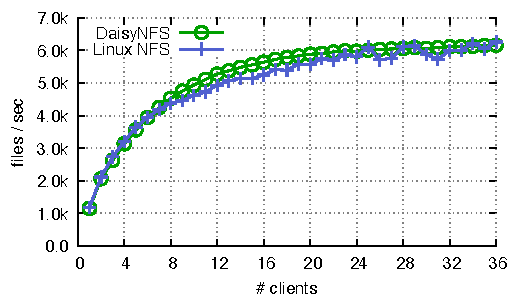
\includegraphics[scale=0.9]{fig/aws-spectre/scale.pdf}

  \caption{Combined throughput of multiple parallel \cc{smallfile}
    microbenchmarks, each creating files in different directories,
    on an NVMe SSD.}
  \label{fig:scale}
\end{figure}

\begin{figure}[ht!]
  \centering

  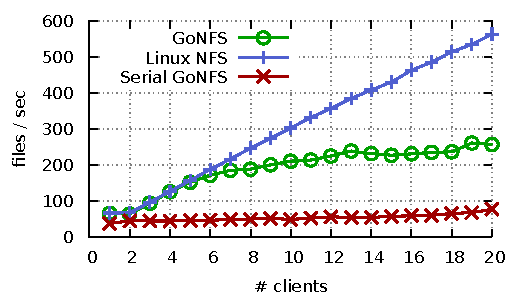
\includegraphics[scale=0.9]{fig/scale.pdf}

  \caption{Combined throughput of multiple parallel \cc{smallfile}
    microbenchmarks, each creating files in different directories,
    on a (slow) SSD.}
  \label{fig:scale-ssd}
\end{figure}

\subsection{Journaling atomicity simplifies proofs}
\label{sec:eval:atomic}

Many storage systems use journaling because they simplify the
implementation in terms of crash safety: the only point at which durable
state is modified is when an operation commits.  A goal of
\txn is to carry this insight into proofs, so that a storage system
using the journal can prove an operation is atomic using reasoning about durable
storage only at the commit point.

One measure of how well \txn achieves this goal is the lines of code in
\simplenfs that require reasoning about durable state.  \simplenfs
consists of \simplenfsLOC{} lines of verified code.  Only \simplenfsCrashLOC{} lines of code require
proofs to explicitly consider durable state, using crash conditions.
In \autoref{fig:write}, for example, crash reasoning is only needed for lines
6--8 when acquiring and releasing with the crash-aware lock specification.  All
of the other
code does not require reasoning about durable state; it suffices to prove
simple crash-free specifications that have a pre- and post-condition, but
no crash condition.  This formal reasoning is enabled by two techniques
from Perennial: lifting disk-object ownership and crash framing.

% \paragraph{Lifting disk-object ownership.}
% Lifting simplifies reasoning about disk-object ownership in \simplenfs in
% two ways.  First, lifting enables \simplenfs to transfer a predicate about
% disk-object ownership into a predicate about in-memory transaction state.
% Subsequent reads and writes within a transaction can operate on the
% transaction state, without worrying about durability until commit.
% Second, lifting enables \simplenfs to transfer predicates about
% disk-object ownership across crashes, to prove that on-disk state is
% correctly preserved on recovery.

% \paragraph{Framing the crash condition.}
% To formally prove that transactions are crash-safe, \simplenfs uses crash
% condition framing.  Specifically, when \simplenfs lifts some predicate
% into a transaction (e.g., a predicate describing the state of the inode),
% the proof immediately uses the durable disk-object ownership to frame
% away the crash-condition obligation until the commit point.  Using the
% durable resources to frame the crash obligation means that the durable
% resources are not available until commit, which in turn proves that they
% are not modified.  At commit time, the resources become available again,
% and the developer must explicitly reason about their crash safety (e.g.,
% just in the code shown in \autoref{fig:writecommit}).


\subsection{Perennial enables modular crash reasoning}
\label{sec:eval:modular}

Atomic crash specifications are crucial for enabling modular reasoning
about crash safety.  In \txn, atomic crash specs are used at many
layer boundaries.  Out of the layers shown in \autoref{fig:layers},
\textsc{circular}, \textsc{wal}, \textsc{obj}, and \textsc{jrnl} all
provide atomic crash specifications, which are used by the layer above. One benefit of atomic crash specs is that they
allowed us to develop these layers independently, using the specifications of
lower layers before their implements were fully proven, as one would
expect of any good API.

The modularity in Perennial largely follows the same structure as the code.
\autoref{fig:loc} shows that the \textsc{wal} and \textsc{jrnl} proofs were
split into an atomic transition specification about the code and a proof-only
abstraction on top, but the bulk of the division was due to boundaries in the
code that made the implementation manageable. Using separation logic it was easy
to prove data structures (like the striped lockmap) and individual utility
functions and use their abstract specifications elsewhere in the proof.

\subsection{Proof effort}
\label{sec:eval:proof}

\autoref{fig:loc} shows the lines of code and lines of proof for \txn
and \simplenfs.  The hardest part of \txn lies in the \textsc{wal}
layer, which has significant lock-free concurrency, and requires careful
reasoning about crashes and recovery.  This is reflected in \textsc{wal}'s
relatively high lines of code, lines of proof, and proof:code ratio.
In contrast,
\simplenfs leverages GoJournal's atomicity, and ends up with a
much smaller proof relative to its code size.


\subsection{Verification prevents bugs}
\label{sec:eval:bugs}

% When developing \simplenfs and
% \txn, we wrote extensive unit tests, but they were not sufficient to
% find all bugs before proving.  When proving \simplenfs, we discovered
% several bugs due to uncaught integer overflows (which wrap around in Go) and
% out-of-bounds reads and writes that could have led to file-system corruption
% (e.g., if the write RPC includes an offset and count that, if added together in
% 64-bit arithmetic, overflows to a value less than the current size of
% the file).

When developing \txn, we wrote unit tests to quickly find problems before starting
verification, but they did not catch all bugs. While proving
\txn, we found a subtle bug in absorption.  When appending a new
transaction in memory, \txn has an optimization called absorption where earlier
writes to the same address are replaced with the new values. However, we discovered a race condition,
where the logger thread could have been already flushing those earlier
writes to disk, leading to unpredictable disk contents depending on the
order of absorption vs logging.  We fixed this issue by introducing the
\cc{nextDiskEnd} boundary, as shown in \autoref{fig:log}: the logger thread only
logs up to \cc{nextDiskEnd}, and absorption is only allowed to modify values
after \cc{nextDiskEnd}.


% Caught a bug where a variable got changed and then we read the new value: \url{https://github.com/mit-pdos/goose-nfsd/commit/255a1c4cc}.
% Forgot to check for out-of-bounds: \url{https://github.com/mit-pdos/goose-nfsd/commit/5cb7b82b9c809}
% Couple missing overflow checks: \url{https://github.com/mit-pdos/goose-nfsd/commit/f5d41e3926c2}, \url{https://github.com/mit-pdos/goose-nfsd/commit/31cc9dcc1}
% Check for inode read past end: \url{https://github.com/mit-pdos/goose-nfsd/commit/b91113936d27}
% added an optimization to make the proof easier: \url{https://github.com/mit-pdos/goose-nfsd/commit/a788305ba0d7}
% introduced data structure (sliding) for mem log to make verification more modular
% introduced layer for on-disk circular log to make verification more modular

% \mfk{describe trusted computing base somewhere: here or in system overview?}
